\documentclass{article}

\usepackage{tikz}

\begin{document}

\begin{center}
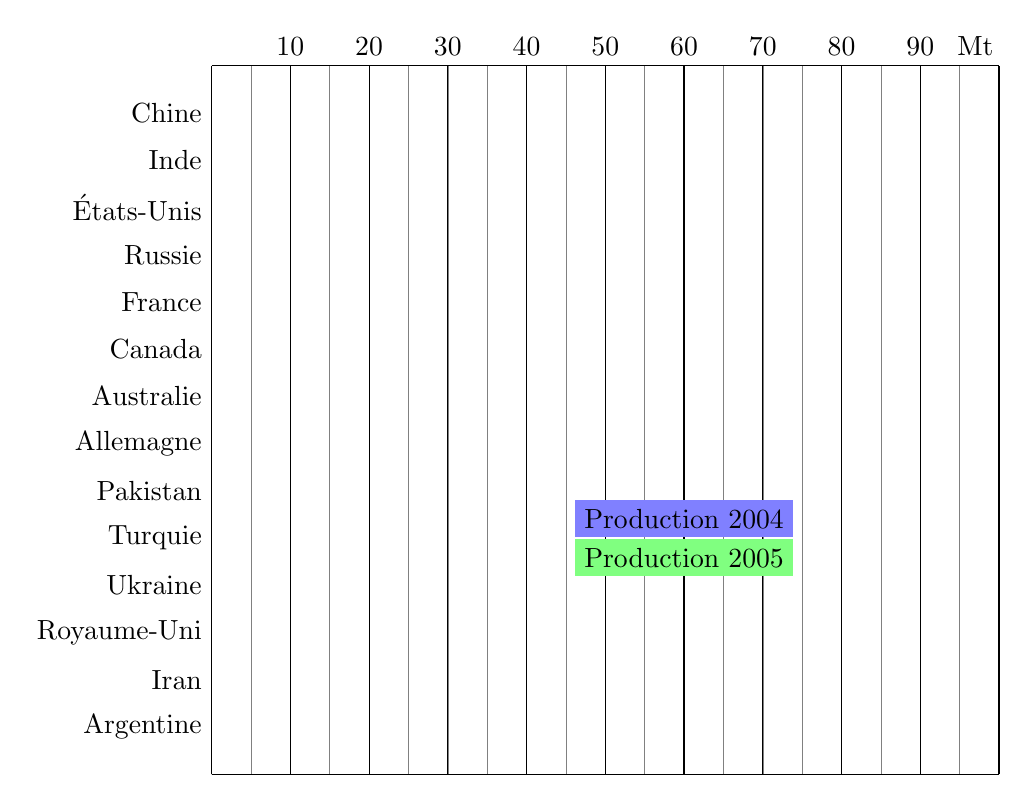
\begin{tikzpicture} [xscale=0.1, yscale=0.6]
  \draw[gray,very thin] (0,0) grid[xstep=5,ystep=15] (100,15);
  \draw (0,0) grid[xstep=10,ystep=15] (100,15);
  \draw[line width=3mm,color=blue!50,yshift=2mm] plot[xcomb]
       file {producBle2004.txt};
  \draw[line width=3mm,color=green!50,yshift=-2mm] plot[xcomb]
       file {producBle2005.txt};
  \foreach \n/\y in {Chine/14,Inde/13,\'Etats-Unis/12,Russie/11,France/10,
       Canada/9,Australie/8,Allemagne/7,Pakistan/6,Turquie/5,Ukraine/4,
       Royaume-Uni/3,Iran/2,Argentine/1}
     \draw (0,\y) node [left] {\n};
  \foreach \x in {10,20,...,90} \draw (\x,15) node[above] {\x};
  \draw (97,15) node[above]{Mt};
  \draw (60,5) node[fill=blue!50,above]{Production 2004};
  \draw (60,5) node[fill=green!50,below]{Production 2005};
\end{tikzpicture}

Les principaux pays producteurs de bl\'e (en millions de tonnes)
\end{center}

\end{document}
